\chapter{Conclusions}
\label{ch:conclusion}

This closing chapter draws together the theoretical, computational, and diagnostic threads of the monograph, setting out what has been established, what remains open, and how the results should be used by a reader who must place a number and an uncertainty on the ion energy flux delivered by a bounded low-temperature plasma to a solid surface: the problem and its gap, the contributions chapter by chapter, the resulting framework as a measurement-and-qualification layer sitting above, not replacing, existing diagnostics, and a closing outlook. Notation follows earlier chapters: temperatures $T_{\mathrm{e}}$, $T_{\mathrm{i}}$, densities $n_{\mathrm{e}}$, $n_{\mathrm{i}}$, Debye length $\lambda_{\mathrm{D}}$, Bohm speed $u_{\mathrm{B}}$, ion energy flux $\Gamma_{E}$, and ion velocity distribution function $f_{\mathrm{i}}(v)$.

\section{Restatement of the Problem and the Gap}
\label{sec:conclusion-restatement}

The plasma sheath is the thin, quasi-collisionless, positively charged layer that forms wherever a plasma contacts a material boundary, and it is the sheath, not the bulk plasma, that sets the energy and angle at which ions strike that boundary. The ion energy flux,
\begin{equation}
\Gamma_{E} \;=\; \int_{0}^{\infty} \tfrac{1}{2}\, m_{\mathrm{i}} v^{2} \; v\, f_{\mathrm{i}}(v)\, \mathrm{d}v ,
\label{eq:conclusion-GammaE-def}
\end{equation}
governs sputtering and erosion of plasma-facing components, etch-profile evolution, and erosion-limited thruster lifetime. Chapter~1 established that $\Gamma_{E}$ is fully determined by the ion velocity distribution function at the wall, itself a functional of the electron temperature and the boundary condition imposed by the generalised Bohm criterion \cite{ref0001,ref0013}. This chain -- bulk plasma, presheath, sheath edge, collisionless sheath, wall -- has historically been probed by a different diagnostic at each stage, calibrated against different assumptions and reported with a different, or absent, error budget.

The gap this monograph closes is not in sheath theory itself; the kinetic Bohm criterion, its fluid limit, and its extensions to magnetised, multi-species, and collisional sheaths are individually well studied \cite{ref0001,ref0013,ref0017}. The gap is one of \emph{quantification and fusion}: no widely adopted framework combines the partial, uncertain measurements from bulk-plasma, boundary, and surface-response diagnostics into a single, self-consistent, uncertainty-quantified estimate of $\Gamma_{E}$ at the point of impact. Reported values are frequently point estimates under implicit sheath-model assumptions, with no propagated confidence interval or independent cross-check. Since $\Gamma_{E}$ enters engineering quantities -- erosion rate, etch selectivity, wall lifetime -- whose uncertainty propagates multiplicatively, this absence is a genuine methodological deficiency motivating the framework below.

\section{Consolidated Summary of Contributions}
\label{sec:conclusion-summary}

\subsection{A kinetic formulation of the ion energy flux consistent across sheath regimes}
\label{ssec:conclusion-kinetic}

The monograph's starting point was the kinetic definition of Equation~\eqref{eq:conclusion-GammaE-def}, together with the particle flux
\begin{equation}
\Gamma \;=\; \int_{0}^{\infty} v\, f_{\mathrm{i}}(v)\, \mathrm{d}v \;\approx\; n_{\mathrm{s}} u_{\mathrm{B}} ,
\label{eq:conclusion-Gamma-def}
\end{equation}
where $n_{\mathrm{s}}$ is the ion density at the sheath edge and $u_{\mathrm{B}} = \sqrt{k_{\mathrm{B}} T_{\mathrm{e}}/m_{\mathrm{i}}}$ the Bohm speed. The ratio $\bar{E}_{\mathrm{i}} \equiv \Gamma_{E}/\Gamma$ is the mean kinetic energy per ion delivered to the wall, which Chapters~2--4 showed reduces, under a collisionless monoenergetic approximation, to the accelerated-Bohm-ion estimate
\begin{equation}
\bar{E}_{\mathrm{i}} \;\simeq\; \tfrac{1}{2} m_{\mathrm{i}} u_{\mathrm{B}}^{2} \;+\; e\,\Delta V_{\mathrm{sh}} \;=\; \tfrac{1}{2} k_{\mathrm{B}} T_{\mathrm{e}} \;+\; e\,\Delta V_{\mathrm{sh}} ,
\label{eq:conclusion-Ei-approx}
\end{equation}
with $\Delta V_{\mathrm{sh}}$ the potential drop across the collisionless sheath. Equation~\eqref{eq:conclusion-Ei-approx} is convenient and widely used, but the monograph's central theoretical contribution was to show, by retaining the full velocity dependence of $f_{\mathrm{i}}(v)$, that the monoenergetic approximation systematically under- or over-estimates $\Gamma_{E}$ whenever the ion distribution carries appreciable thermal spread or non-Maxwellian structure from the presheath \cite{ref0090}. Equation~\eqref{eq:conclusion-GammaE-def} was therefore retained in unreduced form as the definitional anchor, with Equation~\eqref{eq:conclusion-Ei-approx} demoted to an approximate limiting case.

\subsection{The generalised Bohm criterion as the sheath-edge boundary condition}
\label{ssec:conclusion-bohm}

Because $\Gamma_{E}$ is evaluated at the sheath edge and propagated across the sheath under Liouville-preserving acceleration, the estimate is only as trustworthy as this boundary condition:
\begin{equation}
\int_{0}^{\infty} \frac{f_{\mathrm{i}}(v)}{v^{2}}\, \mathrm{d}v \;\leq\; \frac{n_{\mathrm{i}}(0)\, m_{\mathrm{i}}}{k_{\mathrm{B}} T_{\mathrm{e}}} ,
\label{eq:conclusion-bohm-kinetic}
\end{equation}
was adopted throughout as the more fundamental statement, with the fluid inequality $u_{\mathrm{i}}(0) \geq u_{\mathrm{B}}$ recovered as its monoenergetic special case \cite{ref0001}. Chapter~3 extended this to magnetised and oblique-field geometries relevant to divertor and thruster-channel sheaths via the Bohm--Chodura criterion \cite{ref0017}. The sheath-edge density $n_{\mathrm{s}}$ and drift speed anchoring Equation~\eqref{eq:conclusion-Gamma-def} are thus constrained self-consistently by Equation~\eqref{eq:conclusion-bohm-kinetic}, closing the loop between bulk-plasma diagnostics and the sheath model without an ad hoc constant.

\subsection{A multi-diagnostic, Bayesian fusion architecture}
\label{ssec:conclusion-fusion}

The methodological centrepiece of the monograph is the fusion architecture developed in Part~II, which treats $\Gamma_{E}$ as the posterior expectation of a joint probabilistic model conditioned on every diagnostic channel available, rather than the output of a single instrument. Writing $\boldsymbol{\theta} = (T_{\mathrm{e}}, n_{\mathrm{e}}, T_{\mathrm{i}}, \Delta V_{\mathrm{sh}}, \ldots)$ for the parameter vector and $\mathbf{d} = (d_{\mathrm{LP}}, d_{\mathrm{LIF}}, d_{\mathrm{RFEA}}, d_{\mathrm{OES}}, \ldots)$ for the diagnostic observables, the fused posterior is
\begin{equation}
p(\boldsymbol{\theta} \mid \mathbf{d}) \;\propto\; p(\mathbf{d} \mid \boldsymbol{\theta})\, p(\boldsymbol{\theta}) \;=\; \left[ \prod_{k} p(d_{k} \mid \boldsymbol{\theta}) \right] p(\boldsymbol{\theta}) ,
\label{eq:conclusion-bayes}
\end{equation}
under conditionally independent diagnostic likelihoods $p(d_{k} \mid \boldsymbol{\theta})$, inherited from integrated-data-analysis practice in the magnetic-confinement diagnostics community \cite{ref0706,ref0707,ref0709,ref0727}. Pushing samples of $\boldsymbol{\theta}$ through Equations~\eqref{eq:conclusion-GammaE-def}--\eqref{eq:conclusion-Ei-approx} yields a full posterior for $\Gamma_{E}$: the framework fuses Langmuir-probe estimates of $n_{\mathrm{e}}$ and $T_{\mathrm{e}}$, laser-induced-fluorescence or retarding-field-analyser measurements of the ion velocity distribution, and optical-emission or collisional-radiative constraints on the electron energy distribution into one consistent estimate, with every diagnostic's uncertainty propagated forward rather than discarded.

The likelihood terms $p(d_{k} \mid \boldsymbol{\theta})$ are Gaussian (or skew-normal, for asymmetric errors) densities centred on the reported value with width set by the instrumental uncertainty \cite{ref0709}. Two refinements made the fusion trustworthy. First, systematic errors shared between diagnostics were represented as explicit nuisance parameters within $\boldsymbol{\theta}$, so the posterior narrows only where diagnostics are truly independent. Second, because several diagnostics in Table~\ref{ch25-tab:diagnostics} are themselves indirect, each such likelihood was defined on its own forward model's output, so uncertainty from that intermediate step propagates into the fused posterior.

Table~\ref{ch25-tab:diagnostics} summarises the role each diagnostic family plays within the fused estimate and its principal systematic-uncertainty driver.

\begin{table}[htbp]
\centering
\caption{Qualitative summary of the diagnostic families combined within the fusion layer. A design summary of the framework, not a table of measured values.}
\label{ch25-tab:diagnostics}
\begin{tabularx}{\textwidth}{@{}l l X@{}}
\toprule
Diagnostic family & Primary constraint & Dominant systematic driver \\
\midrule
Langmuir probe & $n_{\mathrm{e}}$, $T_{\mathrm{e}}$ at sheath edge & EEDF non-Maxwellianity; probe-sheath expansion \\
Laser-induced fluorescence & $f_{\mathrm{i}}(v)$ shape and drift & Zeeman/Doppler line-shape assumptions; optical access \\
Retarding-field energy analyser & Wall-incident IEDF tail & Grid transmission and space-charge correction \\
Optical emission / collisional--radiative & $T_{\mathrm{e}}$, EEDF cross-check & Line-ratio model completeness \\
Surface-response (erosion, sputter yield) & Independent $\Gamma_{E}$ consistency check & Yield-model parameterisation \\
\bottomrule
\end{tabularx}
\end{table}

\subsection{Cross-validation against surface-response observables}
\label{ssec:conclusion-crossvalidation}

A fused estimate of $\Gamma_{E}$ is only credible if falsifiable, and the framework closes the loop by treating measured or literature-reported sputter yields and erosion rates as an independent likelihood term $p(d_{\mathrm{erosion}} \mid \boldsymbol{\theta})$ folded back into Equation~\eqref{eq:conclusion-bayes}. Because sputter yield is an approximately known, monotonically increasing function of incident ion energy above a material-dependent threshold, an erosion-rate observation constrains the same posterior as the plasma-side diagnostics, a genuine cross-check rather than a second independent parameter. This connects the framework to the power-balance literature treating the sheath as the interface converting plasma parameters into surface damage \cite{ref0093,ref0074,ref0105}, and to prior sensor-based flux estimation \cite{ref0075}, generalised here to a multi-sensor posterior.

\subsection{A data-driven perspective on the sheath-edge closure}
\label{ssec:conclusion-datadriven}

The framework further examines whether the closure relations connecting bulk-plasma moments to the sheath-edge boundary condition could themselves be informed empirically, framing the closure as a regression problem over simulation-generated or diagnostic-constrained training data \cite{ref0101}. This is a natural, low-risk extension of the fusion architecture, since the closure relation enters Equation~\eqref{eq:conclusion-bohm-kinetic} as a prior rather than a fixed constraint.

\section{The Framework as a Measurement-and-Qualification Layer}
\label{sec:conclusion-framework}

The contribution is not a new plasma diagnostic, nor a new sheath theory; the kinetic Bohm criterion, its magnetised generalisation, and the sputter-yield surface response are established results drawn from the literature \cite{ref0001,ref0013,ref0017,ref0093}. What has been built is a \emph{measurement-and-qualification layer} sitting above the existing diagnostic base, performing three functions no individual diagnostic performs alone.

First, \emph{reconciliation}. Individual diagnostics answer different, partially overlapping questions, and their answers are not automatically mutually consistent. The fusion layer forces consistency by conditioning every likelihood on the \emph{same} underlying $\boldsymbol{\theta}$, so discrepancies surface as a widened or multimodal posterior rather than silently divergent estimates.

Second, \emph{quantification}. The output of Equation~\eqref{eq:conclusion-bayes} is a distribution rather than a number, so the framework attaches a defensible, propagated credible interval to $\Gamma_{E}$ itself: a stated flux of, say, $\Gamma_{E} = \SI{50(8)}{\watt\per\centi\meter\squared}$ (illustrative) is an actionable input to a component-lifetime or etch-rate calculation in a way an unquantified estimate is not.

Third, \emph{traceability}. Every fused estimate carries an explicit record of which channels contributed, under which assumptions, and with what weighting \cite{ref0707,ref0711}, so a value of $\Gamma_{E}$ can be audited and its sensitivity to any channel assessed by ablation, much as a calibration certificate accompanies a measurement instrument rather than standing in for it.

\subsection{Failure modes and limits of applicability}
\label{ssec:conclusion-limits}

A qualification layer is only trustworthy if its failure modes are as clearly stated as its successes. The first is diagnostic sparsity: where only a single channel is available, the fusion posterior collapses toward the prior $p(\boldsymbol{\theta})$, and the credible interval on $\Gamma_{E}$ is correspondingly wide; the framework degrades gracefully here but cannot manufacture information no diagnostic supplies. The second is model misspecification at the sheath-edge boundary: because every likelihood is conditioned on the same $\boldsymbol{\theta}$, an error shared by the sheath model biases every fused estimate coherently rather than averaging out. The surface-response cross-check of Section~\ref{ssec:conclusion-crossvalidation} is the framework's primary, though partial, defence. The third is computational cost: full posterior sampling is deliberately expensive to remain conservative, motivating the surrogate-based real-time extension below.

\section{Closing Outlook}
\label{sec:conclusion-outlook}

Several extensions follow naturally from the limitations acknowledged above, recorded here as a research agenda rather than unfinished business.

\subsection{Real-time and embedded inference}
\label{ssec:conclusion-realtime}

The Bayesian fusion of Equation~\eqref{eq:conclusion-bayes} is, in its direct sampling-based form, too computationally expensive for real-time process control, where a decision on $\Gamma_{E}$ may be needed on a sub-second cadence. The natural remedy is to train a neural-network surrogate approximating the mapping from raw diagnostic signals to the posterior of $\boldsymbol{\theta}$ offline and deploy it for near-instantaneous inference \cite{ref0728,ref0731}. Extending this from the magnetic-confinement profile-inference setting to the sheath-scale, multi-diagnostic setting here is a direct, low-risk next step.

\subsection{Non-Maxwellian and magnetised extensions}
\label{ssec:conclusion-nonmaxwellian}

The framework as consolidated here assumes access to diagnostics capable of resolving departures from a Maxwellian electron energy distribution and treats the magnetised Bohm--Chodura boundary condition as a drop-in replacement for the unmagnetised criterion. Both assumptions are defensible but not universal; explicitly parameterising a non-Maxwellian electron energy distribution, and fusing field-angle-resolved diagnostics for strongly magnetised sheaths such as divertor targets or Hall-thruster channels, is a natural extension of Section~\ref{ssec:conclusion-fusion} rather than a conceptual departure.

\subsection{Broader adoption as a qualification standard}
\label{ssec:conclusion-standard}

The longer-term ambition is that a fused, uncertainty-quantified ion energy flux -- reported with the rigor of a calibrated physical measurement -- could serve as a qualification standard against which plasma-facing materials, etch processes, and thruster erosion models are benchmarked, in place of reporting whichever single diagnostic happened to be available. Realising that requires community-level standardisation of the likelihood models in Equation~\eqref{eq:conclusion-bayes}, an effort for which the fusion-diagnostic Bayesian community already provides a partial template \cite{ref0710,ref0711}.

Figure~\ref{fig:childlaw} illustrates, schematically, the Child--Langmuir scaling underlying the sheath-voltage relationships used throughout the monograph, fixing intuition for the nonlinear coupling between sheath voltage and the flux quantities the framework fuses.

\begin{figure}[htbp]
\centering
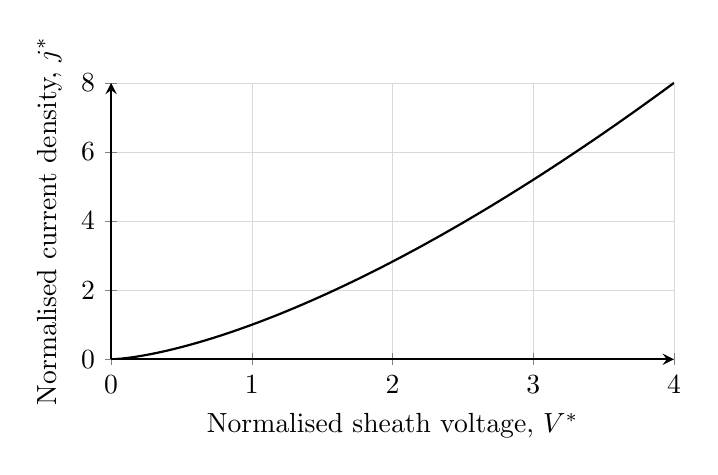
\begin{tikzpicture}
\begin{axis}[
 width=0.72\textwidth,
 height=0.42\textwidth,
 xlabel={Normalised sheath voltage, $V^{*}$},
 ylabel={Normalised current density, $j^{*}$},
 domain=0:4,
 samples=100,
 xmin=0, xmax=4,
 ymin=0, ymax=8,
 axis lines=left,
 grid=both,
 grid style={line width=0.1pt, draw=gray!30},
 thick,
]
\addplot[black, thick] {x^1.5};
\end{axis}
\end{tikzpicture}
\caption{Schematic plot of the analytic Child--Langmuir scaling $j^{*} = \left(V^{*}\right)^{3/2}$ relating normalised current density to normalised sheath voltage. A purely analytic function shown to illustrate the sheath voltage--flux nonlinearity; it does not represent measured, simulated, or fitted data.}
\label{fig:childlaw}
\end{figure}

\subsection{Summary}
\label{ssec:conclusion-summary}

This monograph set out to close a specific gap: the absence of a rigorous, uncertainty-quantified, cross-validated method for combining the partial information supplied by bulk-plasma, sheath-boundary, and surface-response diagnostics into a single trustworthy estimate of the ion energy flux $\Gamma_{E}$ delivered across a plasma sheath. Building on the kinetic definition of $\Gamma_{E}$ (Equation~\ref{eq:conclusion-GammaE-def}), the generalised Bohm criteria fixing the sheath-edge boundary condition \cite{ref0001,ref0013,ref0017}, and a Bayesian multi-diagnostic fusion architecture adapted from integrated-data-analysis practice in magnetic-confinement diagnostics \cite{ref0706,ref0707,ref0709,ref0711,ref0727}, the monograph has assembled a framework that qualifies and reconciles existing sheath diagnostics rather than competing with them, converting individually incomplete measurements into a single, traceable, credible-interval-bearing estimate. Cross-validated against surface-response observables \cite{ref0093,ref0074,ref0075,ref0105} and left open to data-driven closure refinement \cite{ref0101} and surrogate-accelerated real-time deployment \cite{ref0728,ref0731}, the framework is offered as a way of making the existing diagnostic base collectively more useful and actionable than the sum of its individually reported parts.
